\section{Analysis}
In the last section it became clear that the Godot Engine could attract the interest of larger companies.
This already indicates a certain relevance in the video game industry.
However, this does not yet point to the actual question of how relevant the Godot Engine is for indie game developers.
First, we have to define what exactly is meant by indie game development.
Just as the definition of a game engine is elusive, so is the definition of indie game development and indie games developed.
The definition used here is from O'Donnell, which states that indie games focus on a few goals and can be developed on a smaller scale in terms of manpower\cite{indie-definition}.
An indie game development team is not financially supported by a larger company.
This is in contrast to AAA titles, which are developed with high budgets and large teams.\\

For this paper, the digital sales platforms Steam and itch.io were selected for investigation.
On the one hand, this refers to a study by Toftedahl and Engström that provides comparative data from 2018\cite{game-engine-taxonomy}.
On the other hand, reference is made to a survey with 2700 video game developers.
The focus in this paper is on PC and not on console or mobile games.
This is because the survey ``State of the Game Industry'' from 2022 showed that 63\% are actively developing for PC and 58\% plan to do so in the next project as well\cite{gdc-2022}.
In 2019, a survey of video game developers with nearly 4000 participants was conducted\cite{gdc-2019}.
This survey showed that (besides publisher owned and own websites) most games are sold on Steam and itch.io.\\

Without exact details on Steam, it is difficult to track which game engine was used to develop a game.
In the paper by Toftedahl and Engström mentioned above, a script is used that matches the games with articles on Wikipedia and then assigns game engines.
Obviously, this procedure has problems and gaps in the data sets.
This is because not all games have information about the underlying game engine.
There is also another method, which recognizes the used game engines by filenames with the help of pattern matching.
The website SteamDB analyzes the game engines used for development based on this method\cite{steamdb-tech}.
There are problems with this method as well.
Gaps or false positives may exist due to unclear filenames.
In this paper, the datasets from SteamDB are used because matching filenames to game engines seems to be more accurate than matching the data to Wikipedia articles.\\

\begin{table}[h!]
    \centering
    \begin{tabular}{|c c c|}
        \hline
        Game Engine & 2018   & 2022    \\
        \hline\hline
        Unity       & 25.6\% & 61.22\% \\
        Unreal      & 13.2\% & 15.91\% \\
        Source      & 4.0\%  & 0.27\%  \\
        CryEngine   & 3.5\%  & 0.23\%  \\
        GameBryo    & 3.2\%  & 0\%     \\
        IW          & 2.9\%  & 0\%     \\
        Anvil       & 2.5\%  & 0\%     \\
        id Tech     & 1.7\%  & 0.18\%  \\
        Essence     & 1.1\%  & 0\%     \\
        Clausewitz  & 1.0\%  & 0.03\%  \\
        Other       & 48.4\% & 22.17\% \\
        \hline
    \end{tabular}
    \caption{Percentage of total games identified on Steam (data collected 2022-09-30)}
    \label{table:steam}
\end{table}

\autoref{table:steam} shows the percentages of game engines on Steam from 2022 compared to 2018 data.
In fact, with this comparison must be taken with a grain of salt because two different methods have been used.
It is also difficult to say whether the 2022 method can attribute more game engines or simply more games were created using a particular game engine.
This can be explained with the example of Unity.
Unity has 35.62\% more share of all identified games in the last four years.
This could be explained by the pattern matching method capturing more games.
However, it could also be the case that more games in general have been created using the Unity game engine.\textcolor{red}{Steam Graph} \\

\begin{figure}[h!]
    \begin{center}
        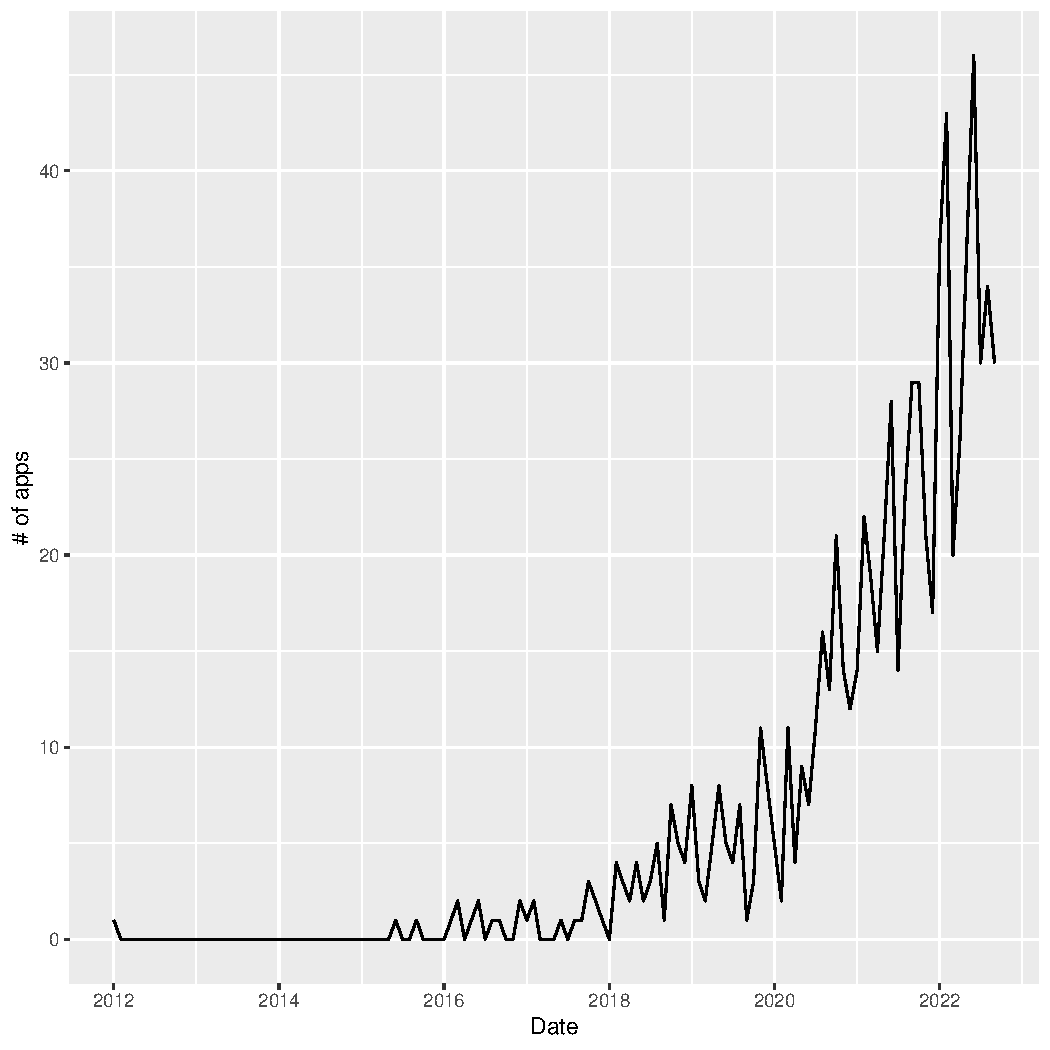
\includegraphics[width=1\columnwidth]{figures/godot-graph.pdf}
        \caption{\label{fig:godot-graph} Number of released Apps on Steam per month}
    \end{center}
\end{figure}

The Godot Engine is not listed in \autoref{table:steam} because the paper providing the comparison data does not list the Godot Engine.
At the time of the collected data, 1.15\% of all games created with the Godot Engine were identified.
Compared to the other game engines on SteamDB, the Godot Engine ranks 7th out of 65 recognized game engines.
So there might be some relevance in the video game industry if the Godot Engine ranks so high.
\textcolor{red}{Graph X shows the games released per month}
If you look at the games released per month, you can clearly see that in 2020, the number of games released has increased significantly.\\

Before examining the reason in more detail, a similar comparison is first made with the data from itch.io.
Compared to Steam, the digital sales platform itch.io mainly features only indie games.
Since this paper focuses exactly on this type of games, this site provides an interesting data set.
Unlike Steam, itch.io has an official statistics website that provides information on game engines\cite{itchio-engines}.
However, this data is unfortunately also incomplete, because this data is self-reported.
So information could be missing or be incorrect here as well.

\begin{table}[h!]
    \centering
    \begin{tabular}{|c c c|}
        \hline
        Game Engine & 2018   & 2022                                                \\
        \hline\hline
        Unity       & 47.3\% & $\textcolor{ForestGreen}{\blacktriangleup 49.75\%}$ \\
        Construct   & 12.3\% & $\textcolor{ForestGreen}{\blacktriangleup 13.12\%}$ \\
        GameMaker   & 11.0\% & $\textcolor{red}{\blacktriangledown 7.32\%}$        \\
        Twine       & 6.2\%  & $\textcolor{red}{\blacktriangledown 5.35\%}$        \\
        RPG Maker   & 3.9\%  & $\textcolor{red}{\blacktriangledown 2.74\%}$        \\
        Bitsy       & 3.3\%  & $\textcolor{red}{\blacktriangledown 3.11\%}$        \\
        PICO-8      & 2.9\%  & $\textcolor{red}{\blacktriangledown 2.68\%}$        \\
        Unreal      & 2.8\%  & $\textcolor{ForestGreen}{\blacktriangleup 2.92\%}$  \\
        Godot       & 2.5\%  & $\textcolor{ForestGreen}{\blacktriangleup 5.55\%}$  \\
        Ren'Py      & 2.0\%  & $\textcolor{red}{\blacktriangledown 1.93\%}$        \\
        Other       & 5.9\%  & $\textcolor{red}{\blacktriangledown 5.55\%}$        \\
        \hline
    \end{tabular}
    \caption{Percentage of total games identified on itch.io (data collected 2022-09-30)}
    \label{table:itch}
\end{table}

Similar to Steam, itch.io data can be compared to the 2018 reference paper.
Since the method used to access the data is the same, a direct comparison can be made.
This comparison can be seen in \autoref{table:itch}.
Game engines that account for a higher percentage of the total games developed in the last four years are highlighted in green.
Game engines that performed worse are highlighted in red.
Comparing the data from \autoref{table:steam} and \autoref{table:itch}, it can immediately be seen that Unity seems to be a popular engine.
Unity accounts for over half of all games on Steam and almost exactly half on itch.io.
This is extremely high when compared to the second-placed game engines, which account for around 16\% on Steam and around 13\% on itch.io.\\

Furthermore, it can be seen that besides Unity, only three other game engines have gained popularity on itch.io.
These three game engines are Construct, Unreal and Godot Engine.
Construct is a game engine primarily aimed at non-programmers.
With the help of visual programming, it is intended to make it easier for novice programmers to get started.
The high percentage could be explained by the fact that many people are interested in developing their own games, but they lack the expertise to do so.
However, this is only an assumption that needs to be investigated further. \\

The Unreal Engine already shows up in \autoref{table:steam} as the second most used game engine on Steam.
However, on itch.io, the Unreal Engine has only gained minimal popularity in the last four years.
This is particularly interesting because it shows that the Unreal Engine has a low relevance among indie game developers.
The Unreal Engine is often referred to as the game engine for AAA games\textcolor{red}{[?]}.
This could be the reason why indie game developers have less interest in it. \\

The Godot Engine has gained a lot of popularity in the last four years.
If you look at the underlying data, it becomes clear that the Godot Engine has more than double the percentage share than before.
To be able to analyze the data even further, a separate script was written, which saves the games from itch.io with their release date as a CSV file.
It should be mentioned that not all games could be fetched with this script.
Despite the missing data sets of up to about 10\%, a trend plot for the game engines from \autoref{table:itch} can still be created.\\

\begin{figure}[h!]
    \begin{center}
        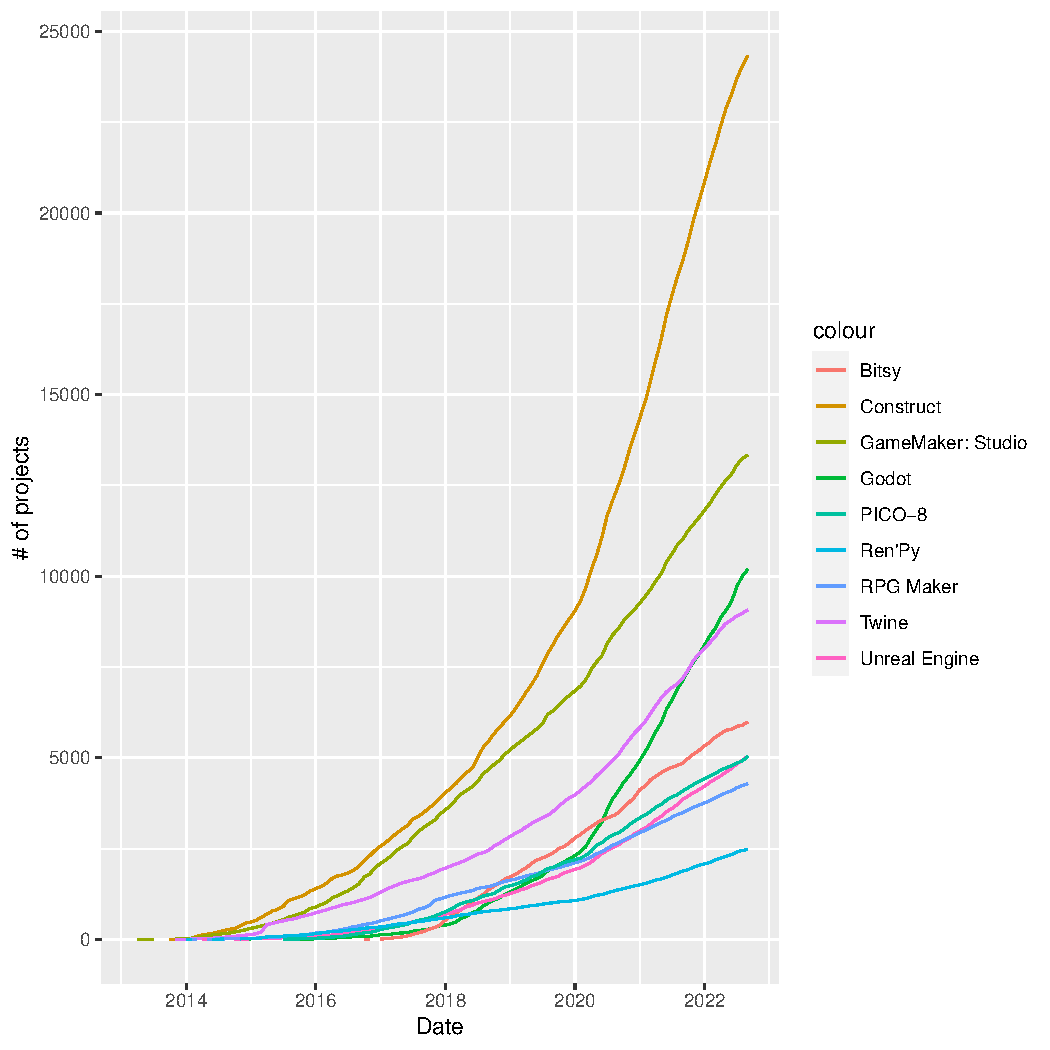
\includegraphics[width=1.3\columnwidth]{figures/trend-graph.pdf}
        \caption{\label{fig:trend-graph} Number of projects on itch.io as trend graph}
    \end{center}
\end{figure}

This graph is shown in \autoref{fig:trend-graph}.
However, Unity has so many projects that the details in the graph would be lost for the other game engines.
For this reason, Unity is not present in the graph.
It is clear to see that the Godot Engine has gained a lot of popularity in 2020, overtaking Bitsy and Twine.
The important observation that emerges here is that both on Steam and on itch.io, more games have been released using the Godot Engine as of 2020.
The reason that more games are released on both platforms may be because developers offer their games for sale on multiple platforms.
Yet, it is quite difficult to determine why exactly the Godot Engine has increased so much in popularity from the beginning of 2020.
This is because there can be numerous factors.
Likewise, important events may have taken place before 2020 that just took longer to make themselves noticeable.
Therefore, only assumptions can be made about the growth in terms of usage on itch.io.
The analysis in this form also reaches its limits, because it is based on the number of games published.
This is because neither the quality nor the number of games published per publisher can be determined.
It is also difficult to say how high the percentage of actual indie game studios is, because not every publisher was analyzed individually.\\

\begin{table}[h!]
    \centering
    \begin{tabular}{|c c c c|}
        \hline
        Game Engine & 2020   & 2021                                               & 2022                                               \\
        \hline\hline
        Unity       & 62.2\% & $\textcolor{red}{\blacktriangledown 61.6\%}$       & $\textcolor{red}{\blacktriangledown 61.1\%}$       \\
        Godot       & 12.2\% & $\textcolor{ForestGreen}{\blacktriangleup 13.1\%}$ & $\textcolor{ForestGreen}{\blacktriangleup 15.6\%}$ \\
        GameMaker   & 10.9\% & $\textcolor{red}{\blacktriangledown 8.9\% }$       & $\textcolor{red}{\blacktriangledown 6.1\%}$        \\
        Unreal      & -      & 4.2\%                                              & $\textcolor{ForestGreen}{\blacktriangleup 4.8\%}$  \\
        Construct   & 1.7\%  & $\textcolor{ForestGreen}{\blacktriangleup 2.4\%}$  & $\textcolor{red}{\blacktriangledown 1.7\%}$        \\
        Stencyl     & 0.1\%  & 0.1\%                                              & -                                                  \\
        Other       & 12.9\% & $\textcolor{red}{\blacktriangledown 6.5\%}$        & $\textcolor{ForestGreen}{\blacktriangleup 7.0\%}$  \\
        No engine   & -      & 3.1\%                                              & $\textcolor{ForestGreen}{\blacktriangleup 3.7\%}$  \\
        \hline
    \end{tabular}
    \caption{Used game engines by GMTK Game Jam participants over the years\cite{gmtk-twitter}}
    \label{table:gmtk}
\end{table}

On itch.io there are many games, which were created during a game jam.
Game jams are defined as follows:
\blockquote{A game jam is an accelerated opportunistic game creation event where a game is created in a relatively short timeframe exploring given design constraint(s) and end results are shared publically\cite{game-jam-definition}.}
With around 18,000 - 22,000 participants and around 5,000 - 6,000 submissions, GMTK Game Jam is the largest past game jam event on itch.io\cite{itch-past-jams}.
\autoref{table:gmtk} shows the game engines used by participants in the events from 2020 to 2022.
This table is clearly showing that the Godot Engine is the only game engine from the table to outperform the usage of the previous year two years in a row.
This could be a clue that game jams on itch.io have ensured that the Godot Engine continues to gain relevance.
However, this is also just an assumption.
It is not far-fetched that a general popularity of a game engine also ensures that it is used more often in game jams.\\

To make better assumptions, the Godot Engine can only be compared to other game engines that have gained popularity on itch.io.
The Godot Engine can be classified as a general-purpose game engine, as it covers a wide range of game genres.
According to Toftedahl and Engström, this puts it in the same category as the Unreal Engine and Unity.
Construct, on the other hand, is a special purpose game engine.
In the introduction, it was already explained that game engines should be compared with each other in terms of a specific purpose.
For this reason, Construct should not be included in a comparison.
For such a comparison, a feature matrix, benchmarks or other technical aspects would be interesting.
Unfortunately, this is beyond the scope of this paper and would need to be explored separately.
In this paper, the focus is specifically on the Godot Engine and its importance to the indie game industry.
However, this work can provide the basis for which game engines should be compared with each other with regard to the indie game industry.\\

To explore more about the Godot Engine, the Godot Community Poll from 2022 was examined\cite{godot-poll-results}.
This survey contains 5315 answers with a different set of questions.
When asked about previous experience with other game engines, the top three were Unity (51\%), Other third party engine (30.6\%), and GameMaker (22\%).
With Unity having a strong presence on both Steam and itch.io, it seems natural that developers would have been in contact with the game engine in advance.
It is difficult to make a correct statement about other third party engines, because the game engine would have to be specified for that.
However, a statement, or rather an assumption, can be made about GameMaker.
If you take a closer look at \autoref{table:gmtk}, it becomes clear that GameMaker is the only game engine that has lost an extremely large percentage.
It could therefore be possible that these developers have switched from GameMaker to the Godot Engine.\\

If we look at the data for the usage of the Godot Engine in the poll, we can see that 56.56\% primarily use the Godot Engine for 2D game development.
This is in contrast to the primary usage of 35.22\% in 3D game development.
It can be said that the Godot Engine has the possibility to develop 2D, 3D and especially XR, but it is primarily used for 2D.
This could have several causes.
On one hand, the Godot Engine could provide more functionality for 2D game development than 3D game development.
On the other hand, oftentimes the workload for 3D game development is higher than for 2D game development.
This workload could be a hurdle for indie game developers, which is why they might prefer 2D game development.\\

That the survey is mainly about indie game developers can be seen from the fact that 84\% stated that they use the Godot Engine as a hobby.
9\%, on the other hand, have stated that they work as a full time indie.
If you go by the definition in this paper, hobby developers also belong to indie game developers.
This is because they focus on a few goals, are not financially supported by larger companies and work in small teams.
That this is the case can be seen from the fact that 97.9\% work on their project alone or in a team of up to five people.
Apart from people who do not earn any money with their games (83.7\%), it can also be clearly seen in this survey that the two most represented digital sales platforms are itch.io (7.1\%) and Steam (6\%).
The fact that itch.io performs better than Steam could be another indication that the Godot Engine is more relevant for indie game developers.
However, this is not necessarily the case because there is no other comparative data from other game engines. \\

Regarding the finding that the Godot Engine has increased in relevance in 2020, data can also be found in the survey.
Most people (22.2\%) had already learned about the Godot Engine in 2019.
However, most of them (21.9\%) only started programming with it in the following year 2020.
This confirms the statement that there may have been important events before 2020 that took longer to convince people to develop.
A possible scenario would be an indie game developer who shares his progress on the Godot Engine in individual videos on YouTube.
These videos may have drawn attention to the Godot Engine in 2019.
Since many people were interested in the game engine, the developer may have made the decision to publish a tutorial in 2020, which motivated many people to start developing in the Godot Engine.
Of course, this is only a scenario, and it does not necessarily have to have the direct cause for this occurrence.
This scenario would probably account for only a small percentage.
The other percentages will probably be combined for completely different reasons.
However, it becomes clear to what extent there may be time shifts.


% TODO: Regarding 2020: 
% When did you first hear of Godot?
% When did you start using Godot?